\section{Evaluation}
\label{sec:evaluation}

We evaluate Cudele on a 15 node cluster, partitioned into 8 object storage
servers, 3 metadata servers, and 2 monitor servers. The object storage servers
double as clients which is fine because clients are CPU and memory bound while
object storage servers are disk IO bound. All daemons run as a single process
which is the default setting for Ceph and the nodes have 2 dual core 2GHz
processors with 8GB of RAM. There are three daemons per object storage server
(one for each disk formatted with XFS) and they share an SSD for the journal.
The nodes are running Ubuntu 12.04.4, kernel version 3.2.0-63 but all
experiments run in Docker containers; this makes it easier to tear down and
re-initialize ({\it e.g.}, dropping the kernel cache) for the cluster between
experiments.

This paper adheres to The Popper
Convention\footnote{\url{http://falsifiable.us}}~\cite{jimenez_popper_2016}, so
experiments presented here are available in the repository for this
article\footnote{\url{https://github.com/michaelsevilla/cudele-popper/}}.
Experiments can be examined in more detail, or even re-run, by visiting the
\texttt{[source]} link next to each figure. That link points to a Jupyter
notebook that shows the analysis and source code for that graph, which points
to an experiment and its artifacts.

%\begin{figure*}[tb]
%\centering
%\includegraphics[width=180mm]{graphs/slowdown.png}
%\caption{Compared to the \texttt{create} phase, saving and persisting
%updates (\texttt{create+save} and \texttt{create+save+persist}) experience only
%a 4.79\(\times\) and 8.66\(\times\) slowdown, in the worst case for 100K files.
%In contrast, maintaining \texttt{global} consistency is 905.70\(\times\)
%slower.  The disadvantage of decoupling the namespace is the merge phase where
%updates are applied to the metadata store (\texttt{create+apply}, resulting in a
%905.70\(\times\) slowdown for 100K files.}\label{fig:global-v-decoupled}
%\end{figure*}

\subsection{Cudele Mechanism Performance}

\begin{figure}[tb]
\centering
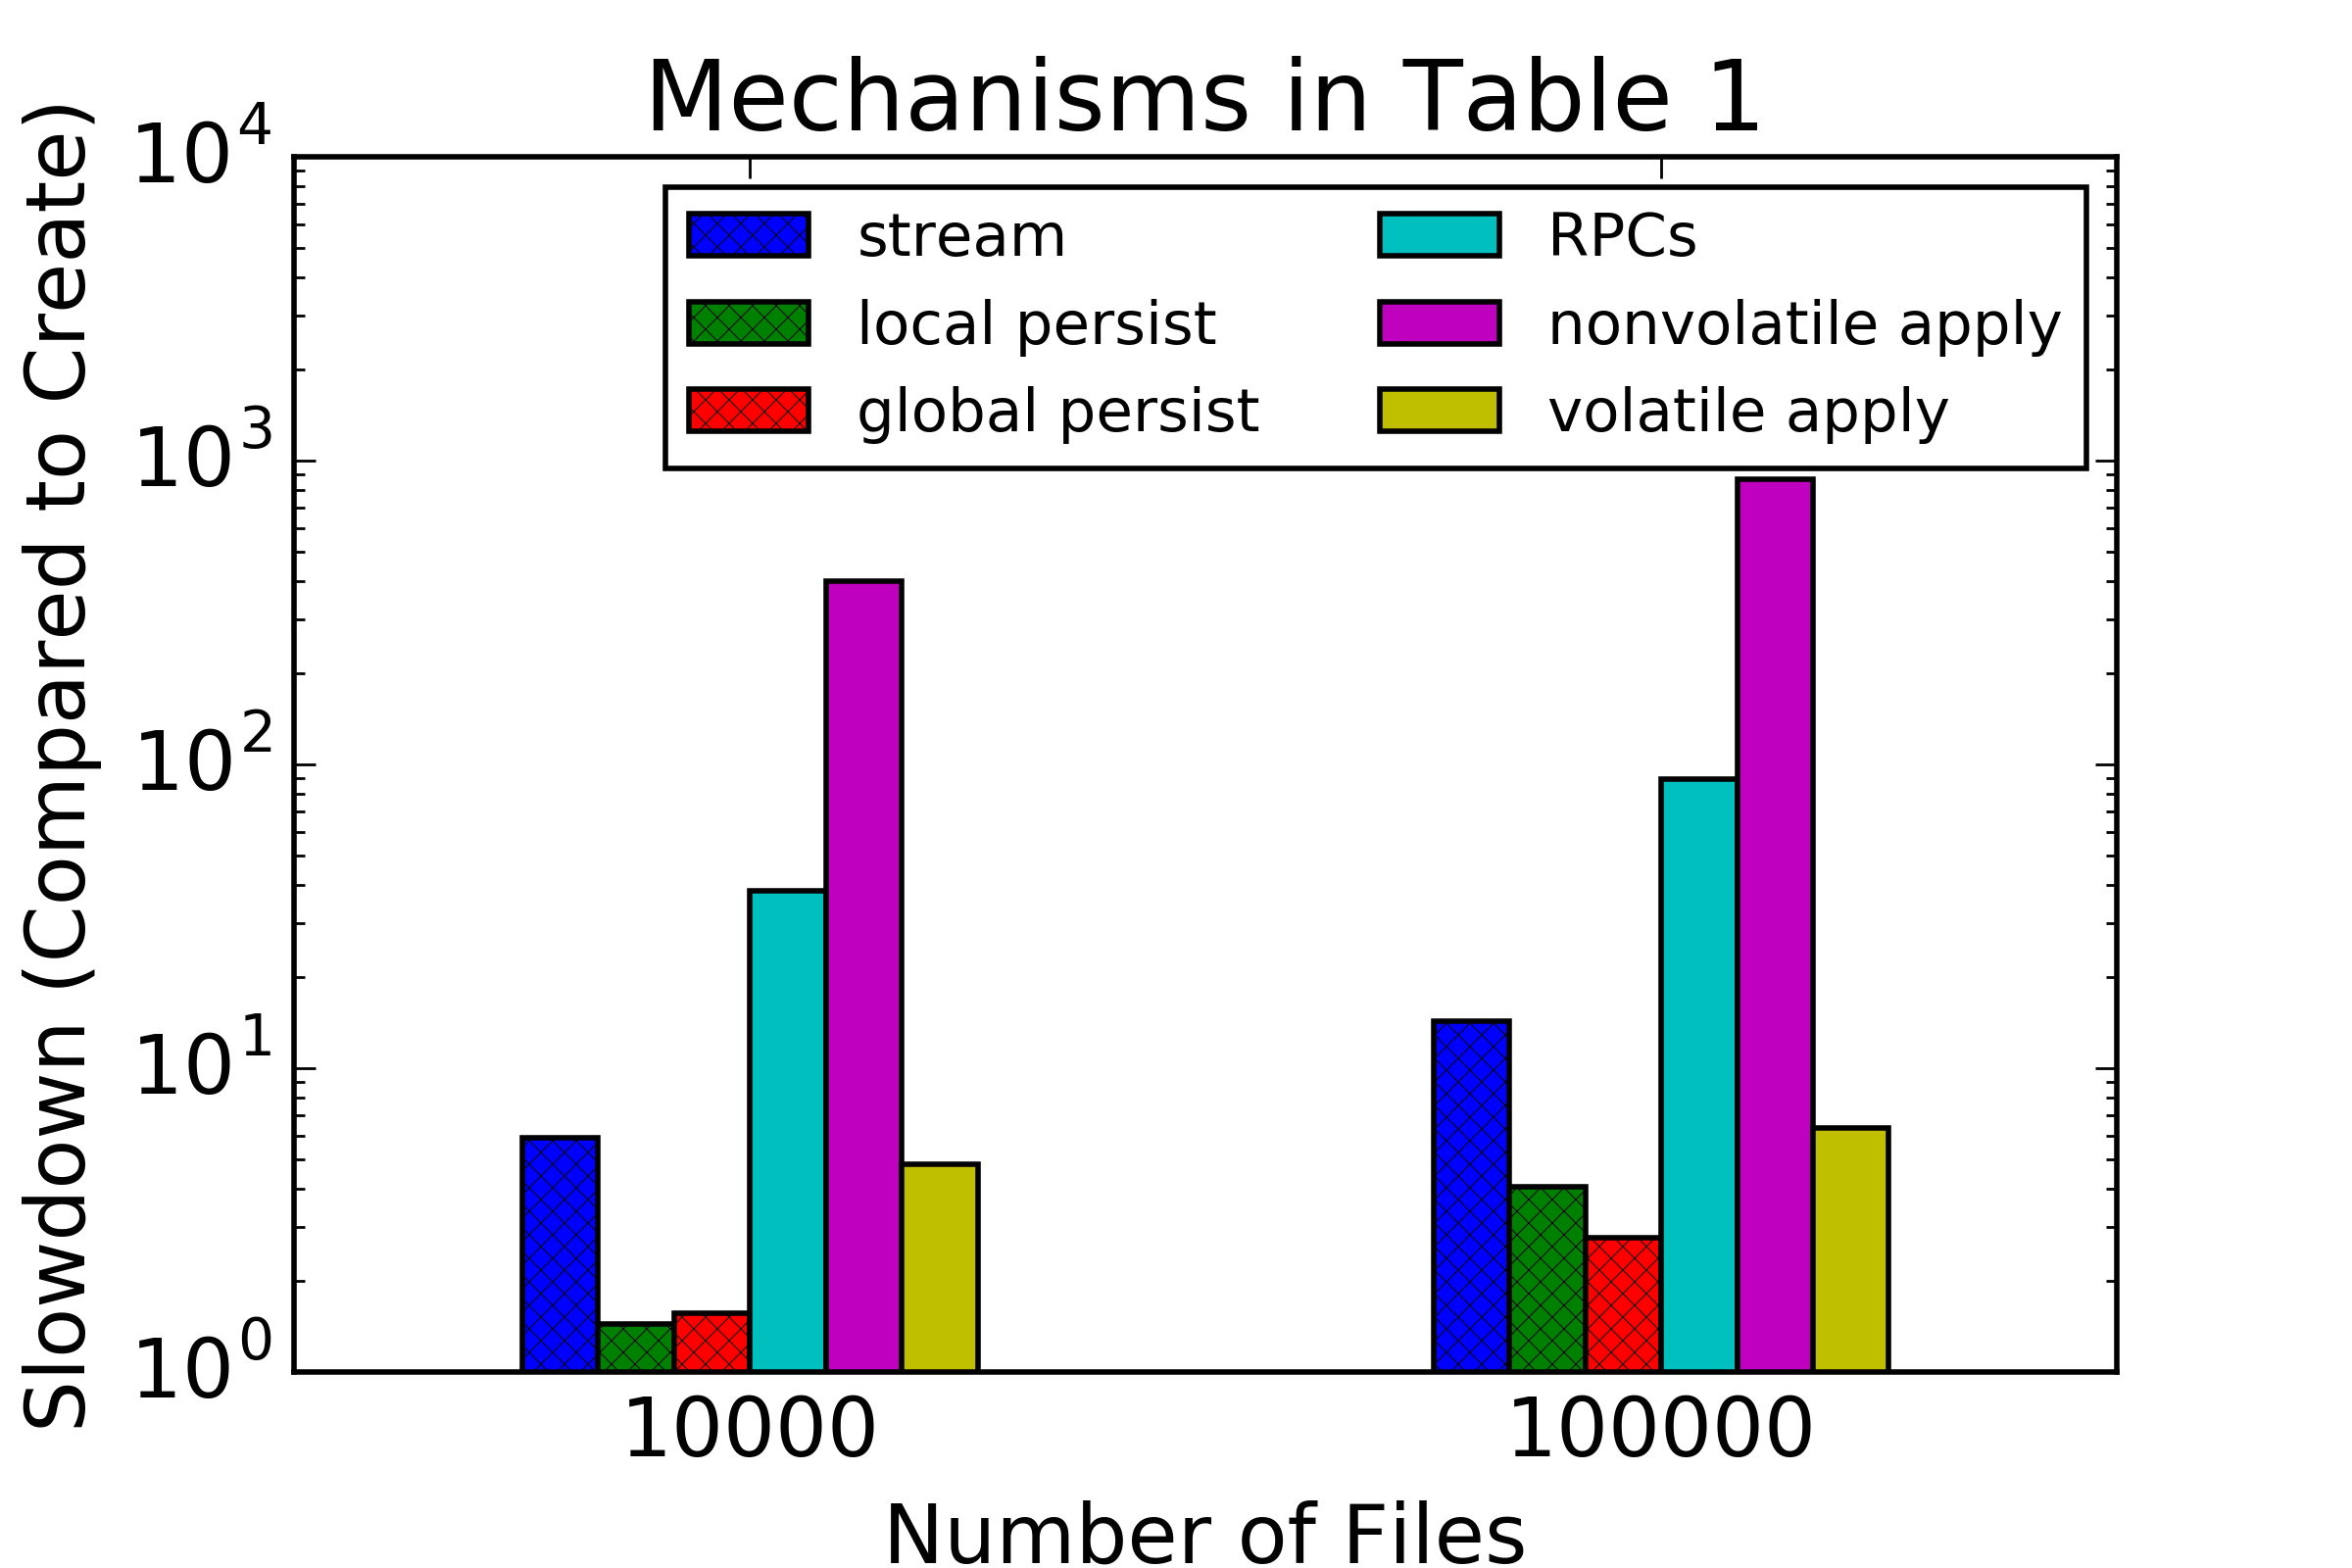
\includegraphics[width=1.0\linewidth]{graphs/slowdown-mechanisms.png}
\caption{
[\href{https://github.com/michaelsevilla/cudele-popper/blob/master/viz-decoupled.ipynb}{source}]
The performance of the Cudele mechanisms normalized to the runtime of the
create mechanism. The runtime of the create mechanism is the time it takes to
write 100 file creates to the client's in-memory journal of metadata
updates.\label{fig:slowdown-mechanisms}}
\end{figure}

\begin{figure}[tb]
\centering
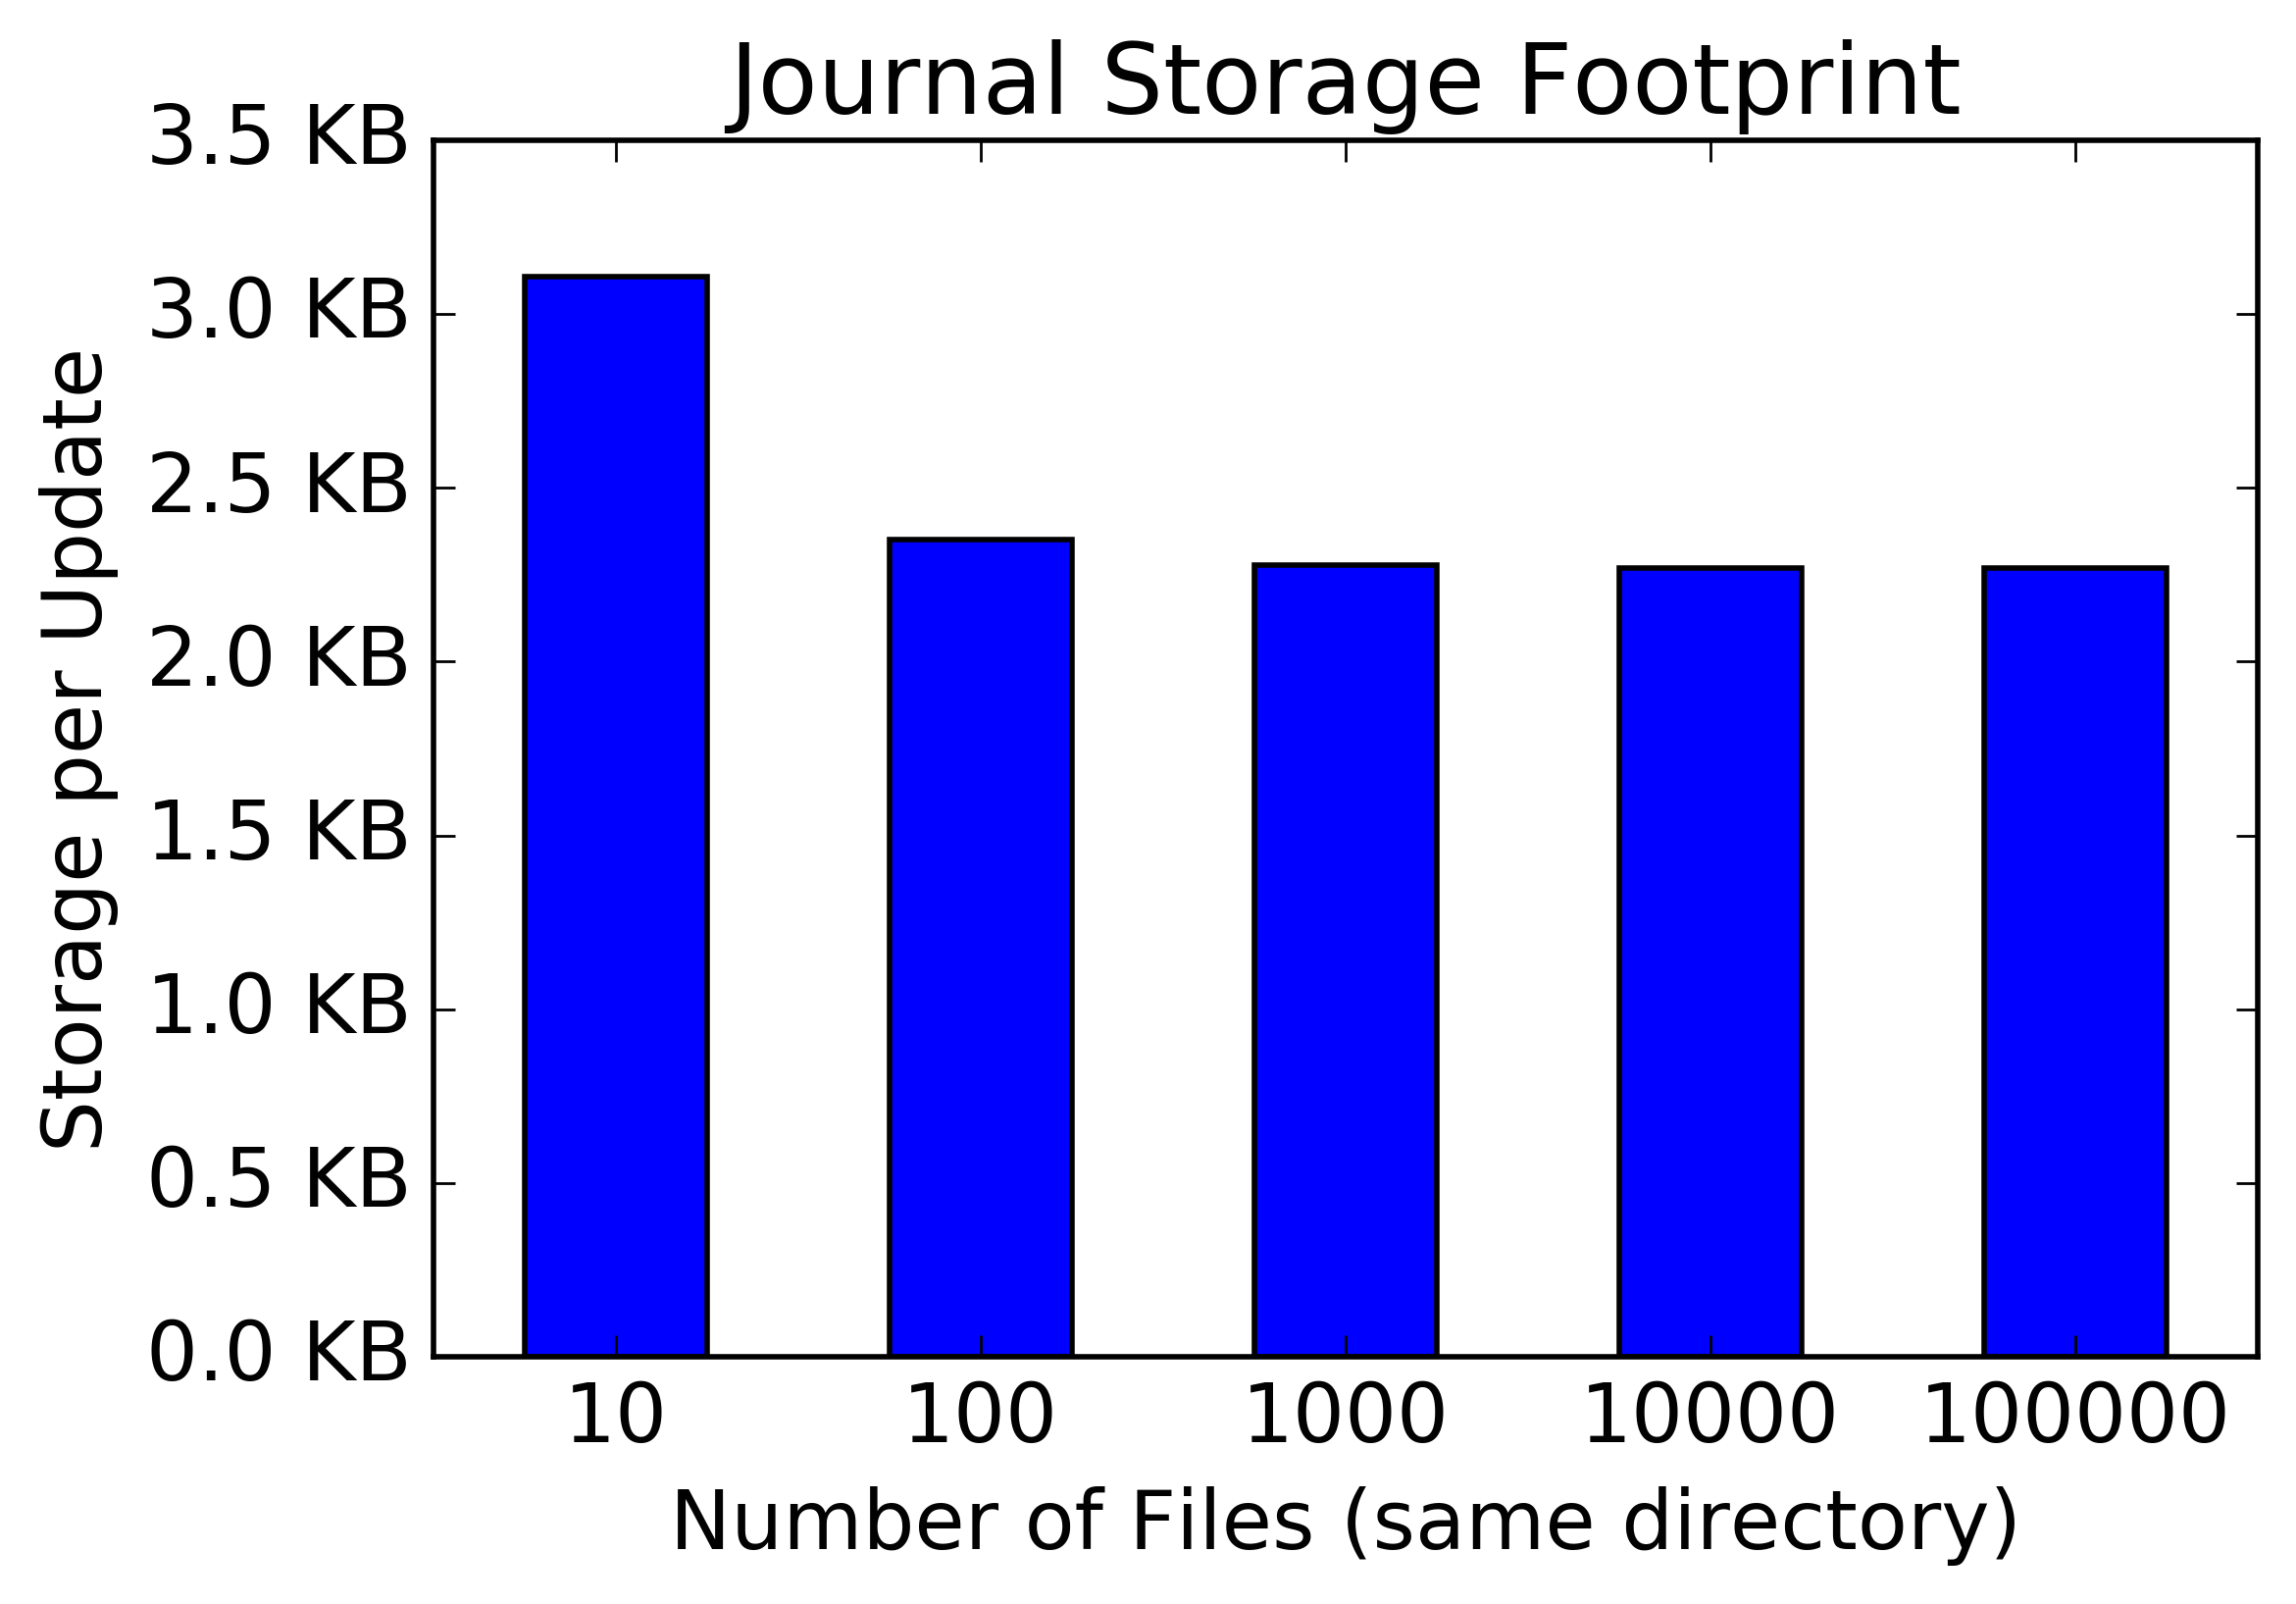
\includegraphics[width=1.0\linewidth]{graphs/behavior-journal-size.png}
\caption{
[\href{https://github.com/michaelsevilla/cudele-popper/blob/master/viz-decoupled.ipynb}{source}]
In-memory client journal scales with the number of
updates.\label{fig:behavior-journal-size}}
\end{figure}

Figure~\ref{fig:slowdown-mechanisms} shows the runtime of the Cudele
mechanisms, normalized to the time it takes to write 100K file create updates
to the client's in-memory journal ({\it i.e.} the create mechanism). Bars above
\(10^0\) are slower than the create mechanism and bars below are faster.
``Stream" is an approximation of the overhead and is calculated by subtracting
the runtime of the job with the journal turned off from the runtime with the
journal turned on. All the slowdowns and speedups reported are for the 100K
file create job, the largest workoad we tested.

% RPCs vs. apply: calls to metadata server vs. RADOS
\subsubsection{Overhead of RPCs} ``RPCs" is \(66\times\) slower than ``volatile
apply" because sending individual metadata updates over the network is costly.
While ``RPCs" sends a request for every file create, ``nonvolatile apply"
writes all the updates to the in-memory journal and applies them to the
in-memory data structures in the metadata server. While communicating the
decoupled namespace directly to the metadata server is faster, communicating
through the object store (``nonvolatile apply") is \(10\times\) slower.

% TODO: why is apply so slow.  
% apply: no CephFS changes, pulls/pushes same RADOS obj.
% v_apply vs. apply/persist: communicating through RADOS
\subsubsection{Overhead of ``nonvolatile apply"} The cost of ``nonvolatile
apply" is much larger than all the other mechanisms.  That mechanism was not
implemented as part of Cudele -- it was a debugging and recovery tool packaged
with CephFS. It works by iterating over the updates in the journal and pulling
all objects that {\it may} be affected by the update.  This means that two
objects are repeatedly pulled, updated, and pushed: the object that houses the
experiment directory and the object that contains the root directory ({\it
i.e.} \texttt{/}).  The cost of communcating through the object store is shown
by comparing the runtime of ``volatile apply" + ``global persist" to
``nonvolatile apply". These two operations end up with the same final metadata
state but using ``nonvolatile apply" is clearly inferior.

% persist vs. save: one disk vs. many
\subsubsection{Parallelism of the Object Store} Comparing ``local" and ``global
persist" demonstrates the bandwidth advantages of storing the journal in a
distributed object store. As the journal size increases, the ``global persist"
performance is \(1.5\times\) faster because the object store is leveraging the
collective bandwidth of the disks in the cluster. This benefit comes from the
object store itself but should be acknowledged when making decisions for the
application; the size of the object store can help mitigate the overheads of
globally persisting metadata updates.

\subsubsection{Journal Size} Figure~\ref{fig:behavior-journal-size} shows the
amount of storage per journal update (\(y\) axis) for the range of file creates
we tested (\(x\) axis). The increase in file size is linear with the number of
metadata creates and suggests that updates for a million files would be
\(2.5\text{KB}*1\text{ million files} = 2.38\text{GB}\). Transfer times for
files this large on an HPC network are reasonable.

\subsection{Weak vs. Strong Consistency}
\begin{figure}[tb]
\centering
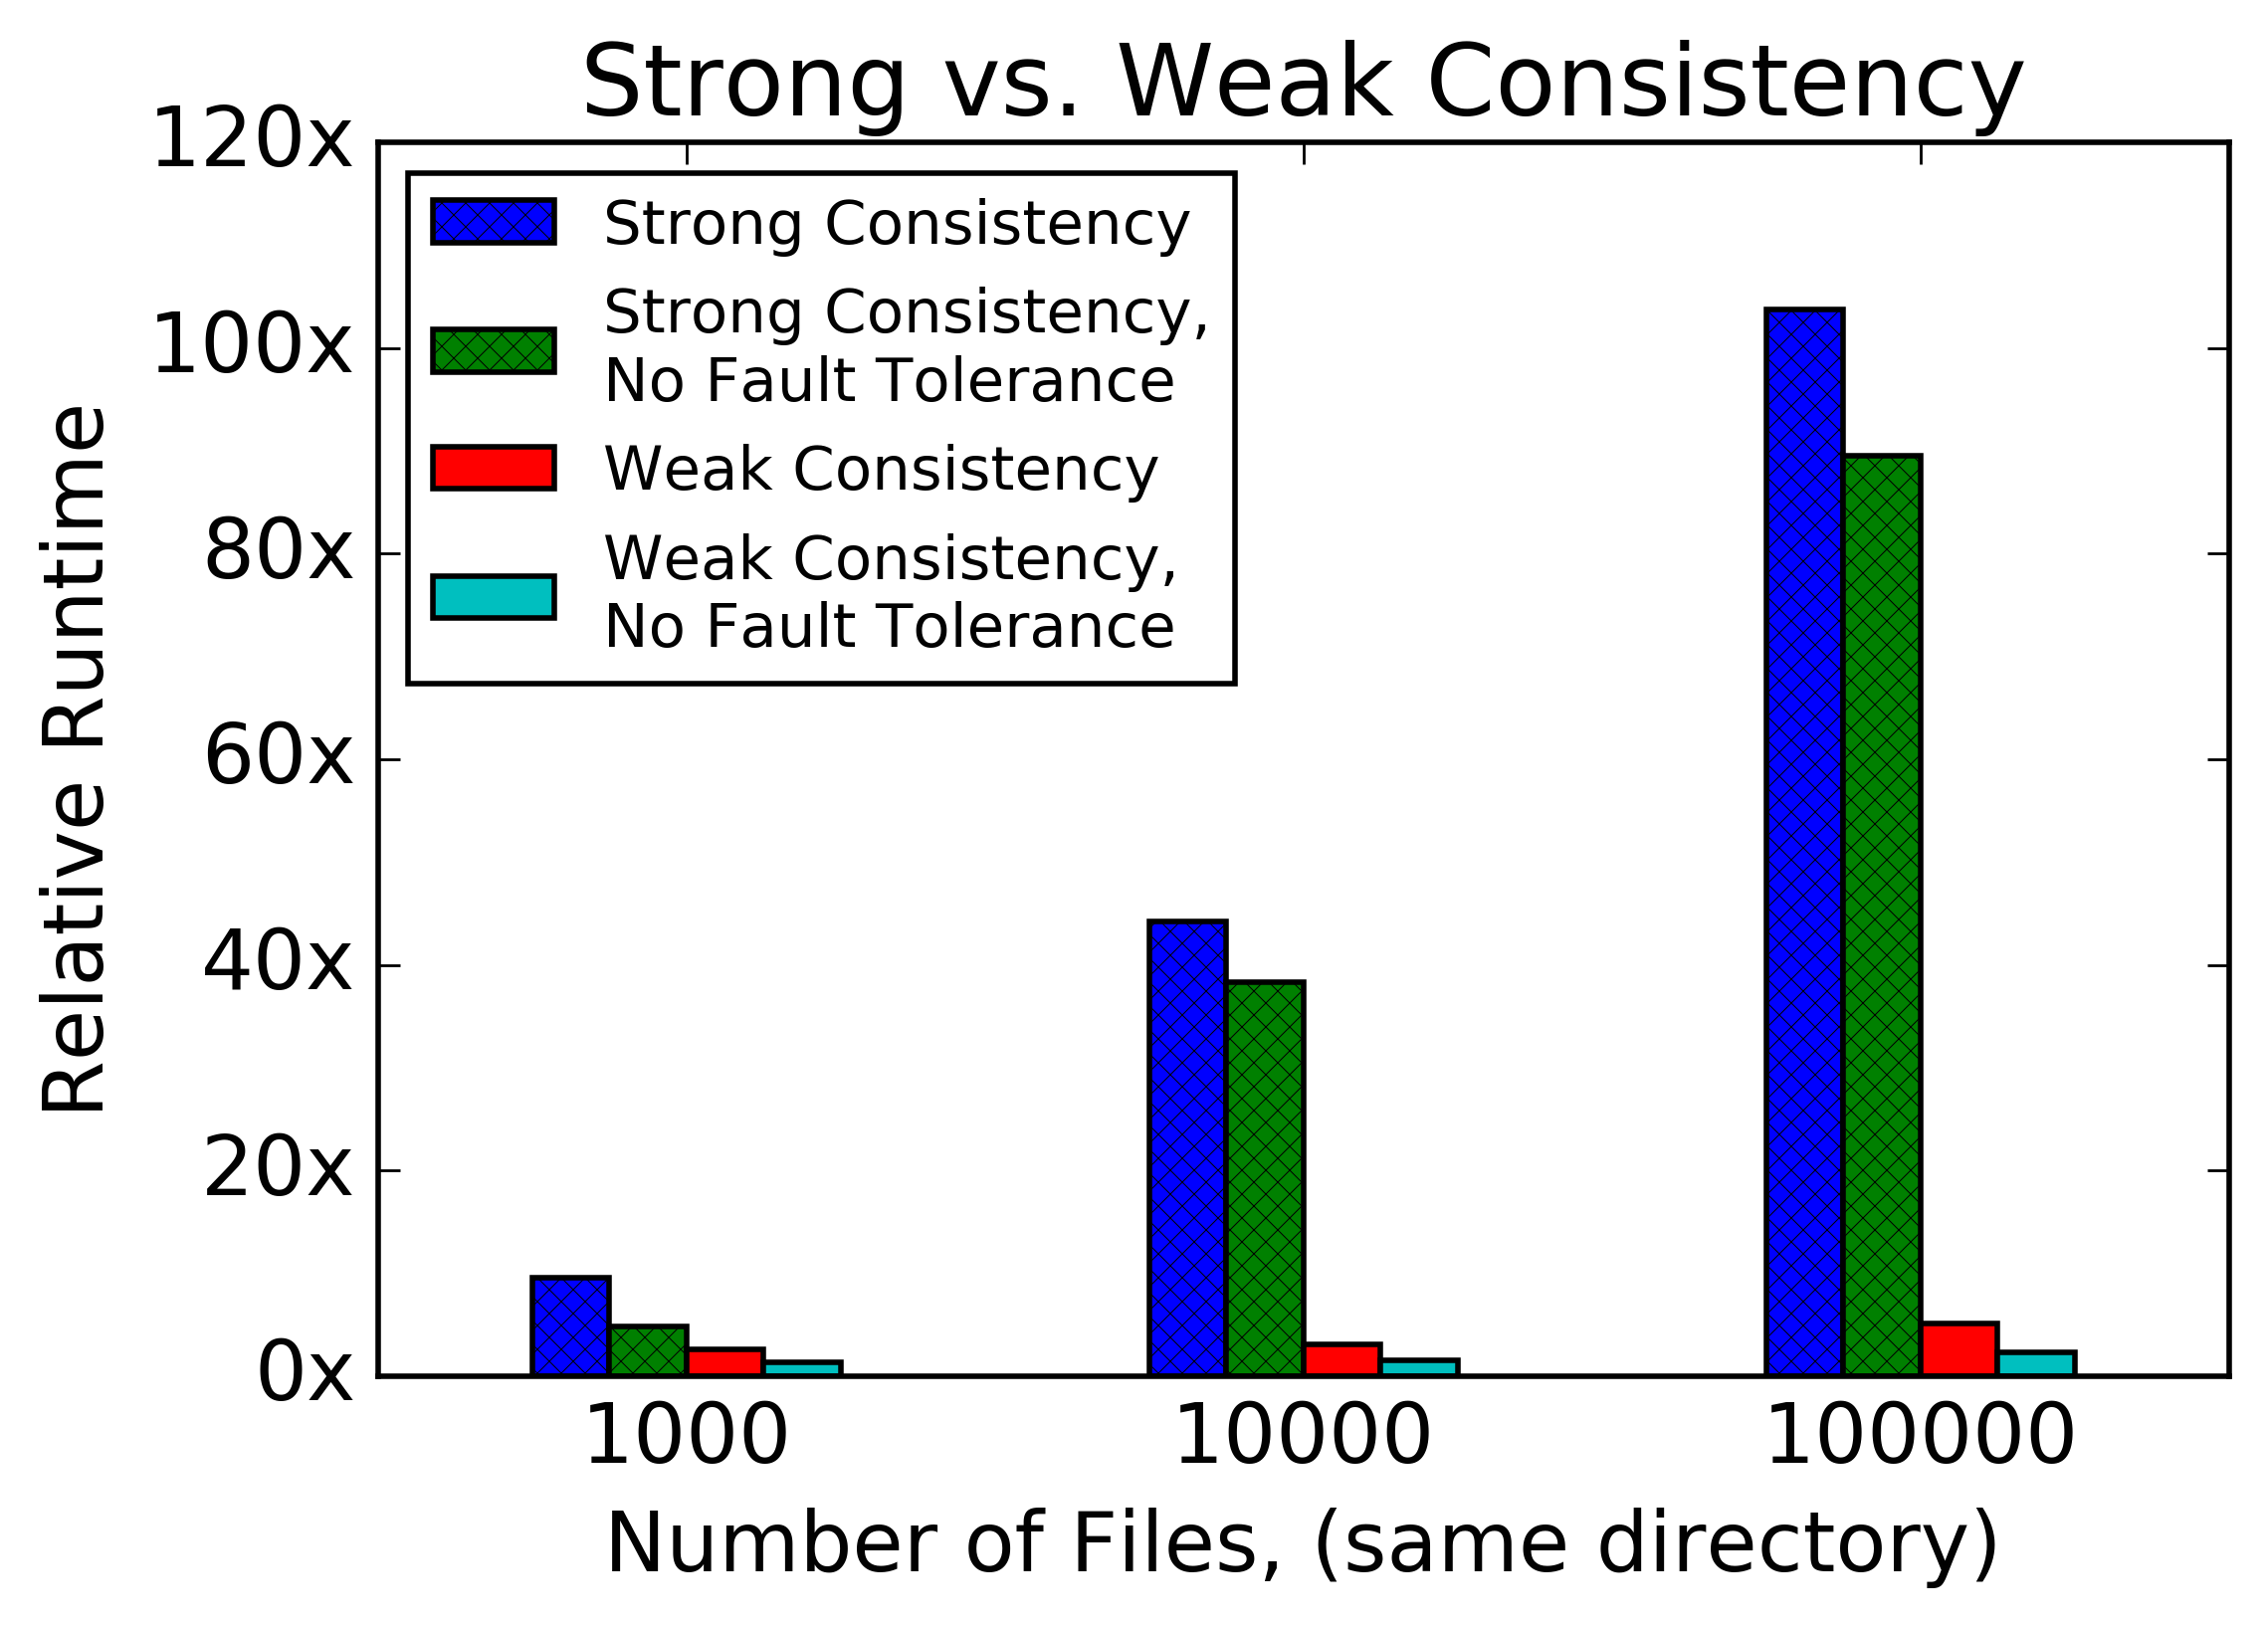
\includegraphics[width=1.0\linewidth]{graphs/slowdown-strong-v-weak.png}
\caption{The RPC per metadata update of ``Strong Consistency" has a large
overhead compared to the decoupled namespace strategy of ``Weak
Consistency".\label{fig:slowdown-strong-weak}}
\end{figure}

Figure~\ref{fig:slowdown-strong-weak} shows the runtimes of weak and
strong consistency based systems implemented on Cudele, normalized to the
runtime of the create mechanism (again, just creating files in the client's
in-memory journal). We scaled the number of files up to 100K which is the
maximum size of a directory by default in CephFS. We use the following
compositions from the mechanisms in Table~\ref{table:spectrum}: 

\begin{itemize}
  \item Strong Consistency
  \begin{itemize}
    \item[]  \texttt{RPCs} \(+\) \texttt{stream}
  \end{itemize}
  \item Strong Consistency, No Fault Tolerance
  \begin{itemize}
    \item[] \texttt{RPCs}
  \end{itemize}
  \item Weak Consistency
  \begin{itemize}
    \item[] \texttt{creates} \(+\) \texttt{local persist}
  \end{itemize}
  \item Weak Consistency, No Fault Tolerance
  \begin{itemize}
    \item[] \texttt{creates} \(+\) \texttt{local persist} \(+\) \texttt{volatile apply}
  \end{itemize}
\end{itemize}

% Final file system metadata states are equivalent No guarantees while
% transitioning mechanisms
We compare these semantics because the final metadata states are equivalent.
Cudele makes no guarantees during execution of the mechanisms or when
transitioning semantics -- the semantics are guaranteed {\it once the mechanism
completes}. So if servers fail during a mechanism, metadata or data may be
lost.

% DeltaFS vs. BatchFS vs. POSIX: decoupled is faster
% (5-7x) vs. (90-104x) slower
% Does not scale?
% Strong Consistency > 10X slower than Weak Consistency 
\subsubsection{Speedups of Decoupled Namespaces} Weak consistency uses the
decoupled namespace strategy and shows up to a \(20\times\) speedup over the
traditional namespaces that use RPCs. Compared to the baseline the slowdown is
\(5-7\times\) for Strong Consistency, which emulates BatchFS and
\(90-104\times\) for Weak Consistency, which emulates DeltaFS.

% POSIX (no stream) vs. POSIX: cost of durability < consistency
\subsubsection{Durability \(<<\) Consistency} The \(1.15\times\) overhead of
``Strong Consistency" compared to ``Strong Consistency, No Fault Tolerance" for
100K files is neglible. It suggests that the overhead of consistency is much
larger than the overhead of durability. This conclusion should be stronger as
we scale the number of files because the cost of streaming the journal into the
object store is constant. We omit the same analysis for ``Weak Consistency"
because the runtimes are so short that the normalized slowdowns are misleading.

% Weak Consistency benefit not due to metadata format
\subsubsection{Metadata Formats} Because the metadata formats are the same for
all schemes we argue that the performance gain for decoupled namespaces comes
from relaxing the consistency guarantees and not from the metadata formats, as
was argued in previous work outlining the benefit of
SSTables~\cite{ren:atc2013-tablefs, ren:sc2014-indexfs}.

%\section{notes}
%Linking clients into our custom libcephfs
%
%Use namespace's recursive data structure to put policies on subtrees
%- consistency: weak vs. strong, global vs. local
%  - e.g., BatchFS/DeltaFS: weak, local
%  - e.g., POSIX: strong, global
%  - e.g., PLFS: no consistency
%- durability: global vs. local
%  - e.g., CephFS: global
%  - e.g., BatchFS/DeltaFS: local
%
%Experimental Setup
%- Ceph: 9 OSDs, 1 metadata server, 2 kernel client
%- Workload limitations: blah
%
%Workload: creates
%
%Baseline: 200K creates in the same directory
%- throughput: degrades at 950s
%- CPU utilization: more at 950s
%- inode cache: eviction dominate
%- inodes +- to cache: eviction dominate
%- per-disk throughput: RADOS not bottleneck
%
%Experiment 1: Interference
%
%\subsection{Baseline}
%Experiment 0: creates in the same directory
%- setup: why we use caching, we use the kernel client, how we circumvent max fragment size
%
%Experiment 0: creates with a stat
%- Hypothesis: metadata read pauses creates and requires a snapshot in time
%  - what is more of an overhead: pausing creates and getting a consistent view OR sucking up resources as it reads from RADOS?
%- can we delay snapshot?
%
%Experiment 1: creates with a readdir
%- Hypothesis: shows the cost of synchronization because on a write, the first client drops his caps
%- client0: create 100k, client1: stat at 2 mins
%
%Experiment 2: scale the number of files
%- See if the open/close spike occurs 
%- Try to see why open/close spike is allowed to happen
%- Try to disable all caching -- metadata writes don't ever re-use the inode -- we never ask for it again!
%- client0: create 100k, client1: touch at 2 mins
%
%Experiment 3: see how fast the cache satisfies a read
%- client0: create 100k, stat inodes
%- client0: create 100k, client1: stat inodes
%
%lient 0: creates, client 1 create(s)

\subsection{Benefits of Isolated Subtree Policies}
% setup: 2cs sep dirs, 2cs DN, 1c malicious write
In this section, we show the isolation benefits of subtree policies.  We repeat
the experiment from Figure~\ref{fig:interfere-b}, where clients write to their
own private directories and another client interferes at 30 seconds.  We also
have 2 clients write to decoupled namespaces and merge their updates 90
seconds.

\subsection{Scaling Concurrent Merges}

\subsection{Partial Directory Listings}

\subsection{Cost of Nonvolatile Apply}
% Why so slow?
Creating many files in the same directory would touch the same object but the
existing implementation results in this object being repeatedly pushed/pulled.


